\subsection{Algorithms Chosen}
\label{sec:choice}

Choosing which algorithms to test is largely intuitive. It is based on the
strengths and weaknesses of different optimization methods within the
algorithms as well as what is being predicted.  

For a benchmarking excercise, some \gls{ML} approaches here were chosen
based on previous work \cite{dayman_feasibility_2013}: nearest neighbor and
ridge regression. These are useful because they are simple, providing
distance-based and linear-based models, respectively. If more complex
algorithms are not required to obtain useful results, then there is no need to
use more computationally expensive options. However, hedging on the fact that
more complex models will be needed, this work also employs an algorithm that is
known to handle highly dimensional data sets well: \acrfull{SVR}.
These algorithms were introduced in Section \ref{sec:algs}. 

\begin{table}[!htb]
  \centering
  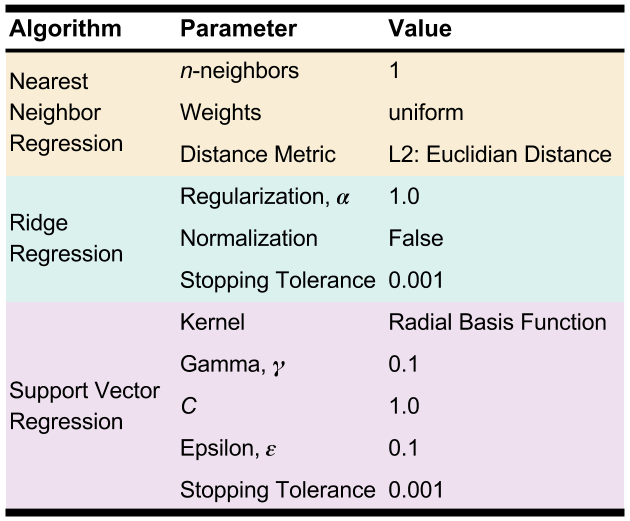
\includegraphics[width=0.8\linewidth]{./chapters/demo_method/defaults.png}
  \caption{Algorithm Parameters Used in Demonstration}
  \label{tbl:defaults}
\end{table}

The parameters chosen for the algorithms are shown in Table \ref{tbl:defaults}.
For many, the default behavior was retained. Prior to training, the data set is
preprocessed by scaling and normalization because the nuclide concentrations
vary by many orders of magnitude. Algorithm implementations from a python-based
\gls{ML} toolkit, scikit-learn \cite{scikit}, are used to train the
models.

\subsection{Reactor Parameter Prediction}
\label{sec:rxtrparam}

The above was carried out, training various statistical models of \gls{SNF}
using nuclide correlations with burnup. As a reminder, this is not the entirety
of the nuclode output from \gls{ORIGEN}; it is the top 200 nuclides by
concentration in each row. Following the training phase, it is important to
estimate the reactor parameter prediction capabilities of those models by
testing their generalizability.  This is done with the previously described set
of measurements from a test data set (shown in Table \ref{tbl:test}) with
samples that mimic potential interdicted \gls{SNF}. The testing set has the
same features as the training set, with known burnup labels that are compared
to the predicted labels. 

\begin{table}[!htb]
  \centering
  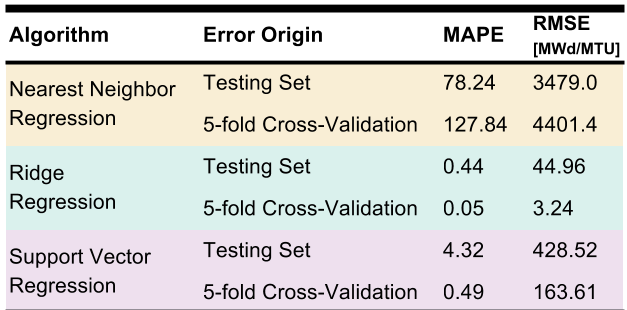
\includegraphics[width=0.8\linewidth]{./chapters/demo_method/results1.png}
  \caption{Three Models' Burnup Prediction Errors}
  \label{tbl:err}
\end{table}

For no introduced error, each model's prediction errors are shown in Table
\ref{tbl:err}.  First, shown here are two \textit{types} of error: the testing
set and via \gls{CV}.  Although previous work uses the former, it is expected
that the latter will provide better estimates of model behavior.  The models
evaluated by the testing set do not have a validation set for pre-evaluation.
The models that are evaluated via \gls{CV} do not use the testing set. 

Table \ref{tbl:err} also includes two error \textit{metrics}.  For the sake of
comparison to previous work and convenient interpretation, \gls{MAPE} is
tracked. However, \gls{MAPE} is not the only error metric. Being that it
approaches infinity near true values of zero, absolute and squared deviations
can also be tracked and may provide more information.  Anecdotally, the
preferred method in the community is to use \gls{RMSE} for model error
estimation, so both are tabulated.  Future work will also track \gls{MAE} since
the nature of the errors are not yet known.  

Regardless, the \gls{MAPE} shows that there are some extremely high and
extremely low errors depending on the algorithm; both results indicate poor
performance with high bias and high variance, respectively.  This is quite
concerning, because these results are from error-free data.

\begin{figure}[!htb]
  \centering
  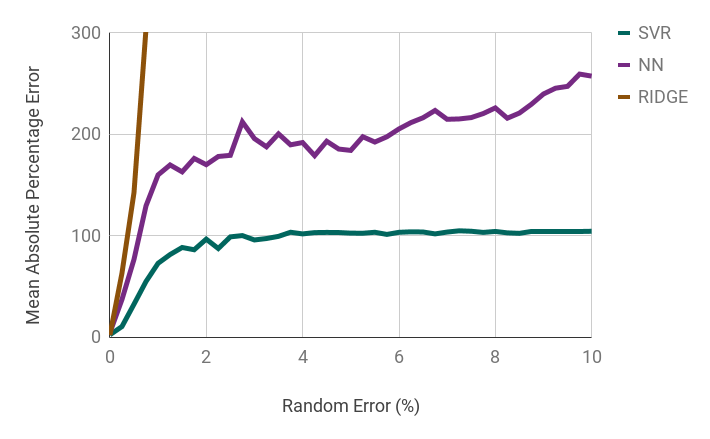
\includegraphics[width=\linewidth]{./chapters/demo_method/randerr.png}
  \caption{Prediction Error from Information Reduction via Random Error}
  \label{fig:randerr}
\end{figure}

Next, information reduction was carried out with all three \gls{ML} approaches.
Figure \ref{fig:randerr} shows the three algorithms' negative \glspl{MAPE} with
respect to the reduction of information by the introduction of random error to
the nuclide vectors, as described in Section \ref{sec:inforeduc}. Negative
errors are used in this work for plotting to abide by the convention of
\textit{`the higher, the better'}.  \gls{SVR} is shown to perform the best, but
it quickly reaches 100\% error. Although ridge regression rapidly increases
with any amount of error, nearest neighbor regression shows more promise,
although it reaches 257\% at 10\% error.  Overall, this performance indicates
that these algorithms are unlikely to predict burnup when faced with the
uncertainties in real-world measurements or the further reduction in
information from gamma detection.

Despite this poor initial performance, the results in Table \ref{tbl:err} and
Figure \ref{fig:randerr} can be evaluated. Next introduced are some diagnostic
and optimization procedures that can shed light on these results.
